%%%%%%%%%%%%%%%%%%%%%%% file template.tex %%%%%%%%%%%%%%%%%%%%%%%%%
%
% This is a general template file for the LaTeX package SVJour3
% for Springer journals.          Springer Heidelberg 2010/09/16
%
% Copy it to a new file with a new name and use it as the basis
% for your article. Delete % signs as needed.
%
% This template includes a few options for different layouts and
% content for various journals. Please consult a previous issue of
% your journal as needed.
%
%%%%%%%%%%%%%%%%%%%%%%%%%%%%%%%%%%%%%%%%%%%%%%%%%%%%%%%%%%%%%%%%%%%
%
\RequirePackage{fix-cm}
%
%\documentclass{svjour3}                     % onecolumn (standard format)
%\documentclass[smallcondensed]{svjour3}     % onecolumn (ditto)
\documentclass[smallextended]{svjour3}       % onecolumn (second format)
%\documentclass[twocolumn]{svjour3}          % twocolumn
%
\smartqed  % flush right qed marks, e.g. at end of proof
%
\usepackage{graphicx}
\usepackage[numbers]{natbib}
\usepackage{bussproofs}
\usepackage{tikz}
\usepackage{amssymb}
\usepackage{amsmath}
\usepackage[all,cmtip]{xy}
\usetikzlibrary{positioning, automata}
\usetikzlibrary{decorations.pathmorphing}

\tikzset{snake it/.style={decorate, decoration=snake}}

\usepackage[T1]{fontenc}
\DeclareFontFamily{T1}{calligra}{}
\DeclareFontShape{T1}{calligra}{m}{n}{<->s*[1.44]callig15}{}
\DeclareMathAlphabet\mathzapf       {T1}{pzc} {mb} {it}


%
% \usepackage{mathptmx}      % use Times fonts if available on your TeX system
%
% insert here the call for the packages your document requires
%\usepackage{latexsym}
% etc.
%
% please place your own definitions here and don't use \def but
% \newcommand{}{}
%
% Insert the name of "your journal" with
% \journalname{myjournal}
%
\begin{document}


\title{(Parallel) Efficient Subclasses Of CFL-Reachability Queries%\thanks{Grants or other notes
%about the article that should go on the front page should be
%placed here. General acknowledgments should be placed at the end of the article.}
}
%\subtitle{Do you have a subtitle?\\ If so, write it here}

%\titlerunning{Short form of title}        % if too long for running head

\author{Ekaterina Shemetova         \and
        Semyon Grigorev %etc.
}

%\authorrunning{Short form of author list} % if too long for running head

\institute{E. Shemetova \at
             St. Petersburg Academic University, ul. Khlopina, 8, Saint Petersburg 194021, Russia, \\ JetBrains Research \\
              \email{katyacyfra@gmail.com}           %  \\
%             \emph{Present address:} of F. Author  %  if needed
           \and
           S. Grigorev \at
              St. Petersburg State University, 7/9 Universitetskaya nab., Saint Petersburg 199034, Russia, \\ JetBrains Research  \\
              \email{s.v.grigoriev@spbu.ru}    
}

\date{Received: date / Accepted: date}
% The correct dates will be entered by the editor


\maketitle

\begin{abstract}
The context-free language (CFL) reachability problem for a context-free grammar $G$ and directed edge-labelled graph $D$ consists of determining for every pair of nodes  $v$ and $u$ whether $v$ can reach $u$ via a path labelled by string in $L(G)$. 
\par
Inspite the 
\keywords{CFL-reachability \and Complexity \and Boolean circuit}
% \PACS{PACS code1 \and PACS code2 \and more}
% \subclass{MSC code1 \and MSC code2 \and more}
\end{abstract}



\section{Introduction}
\label{intro}
The context-free language (CFL) reachability problem is an important problem underlying some fundamential static code analysis \cite*{RepsBasic, Incremental} and graph database query evaluation \cite{HellingsCFPQ}\cite{RDF}\cite{GrigorevRagozina}.
\par
Unlike context-free language recognition, which is in NC, CFL-reachability is P-complete \cite{Yannakakis}\cite{RepSeq}. Practically, it means that we don't have an efficient parallel algorithm for solving this problem (unless $P \neq NC$). But want some cases... . Simple cases (examples, trees etc)... Our focus is on the...
\\This paper is organized as follows.
\section{Preliminaries} \label{section_preliminaries}
In this section, we introduce the basic notions used throughout the paper.

Let $\Sigma$ be a finite set of edge labels. Define an \textit{edge-labeled directed graph} as a tuple $D = (V, E)$ with $V$ is a set of nodes and $E \subseteq V \times \Sigma \times V$ is a directed edge-relation.  For a path $\pi$ in a graph $D$ we denote $l(\pi)$ --- the unique word obtained by concatenating the labels of the edges along the path $\pi$. Also, we write $n \pi m$ to indicate that a path $\pi$ starts at node $n \in V$ and ends at node $m \in V$.

According to Hellings~\cite{hellingsRelational}, we deviate from the usual definition of a context-free grammar in \textit{Chomsky Normal Form}~\cite{chomsky} by not including a special start non-terminal, which will be specified in the queries to the graph. Since every context-free grammar can be transformed into an equivalent one in Chomsky Normal Form and checking that an empty string is in the language is trivial, then it is sufficient to only consider grammars of the following type. A \textit{context-free grammar} is 3-tuple $G = (N, \Sigma, P)$ where $N$ is a finite set of non-terminals, $\Sigma$ is a finite set of terminals, and $P$ is a finite set of productions of the following forms:

\begin{itemize}
    \item $A \rightarrow B C$, for $A,B,C \in N$,
    \item $A \rightarrow x$, for $A \in N$ and $x \in \Sigma$.   
\end{itemize}

Note that we omit the rules of the form $A \rightarrow \varepsilon$, where $\varepsilon$ denotes an empty string. This does not limit the applicability of further algorithms because checking that an empty string belongs to the context-free language in Chomsky normal form is trivial and only the empty paths $m \pi m$ correspond to an empty string $\varepsilon$.

We use the conventional notation $A \xrightarrow{*} w$ to denote that the string $w \in \Sigma^*$ can be derived from a non-terminal $A$ by some sequence of applying the production rules from $P$. The \textit{language} of a grammar $G = (N,\Sigma,P)$ with respect to a start non-terminal $S \in N$ is defined by $L(G_S) = \{w \in \Sigma^*~|~S \xrightarrow{*} w\}$.

For a given graph $D = (V, E)$ and a context-free grammar $G = (N, \Sigma, P)$, we define \textit{context-free relations} $R_A \subseteq V \times V$, for every $A \in N$, such that $R_A = \{(n,m)~|~\exists n \pi m~(l(\pi) \in L(G_A))\}$.

We define a binary operation on arbitrary subsets $N_1 , N_2$ of $N$ with respect to a context-free grammar $G = (N, \Sigma, P)$ as $N_1 \cdot N_2 = \{A~|~\exists B \in N_1, \exists C \in N_2 \text{ such that }(A \rightarrow B C) \in P\}.$

Using this binary operation as a multiplication on arbitrary subsets of $N$ and union of sets as an addition, we can define a \textit{matrix multiplication}, $a \cdot b = c$, where $a$ and $b$ are matrices of the suitable size that have subsets of $N$ as elements, as $c_{i,j} = \bigcup^{n}_{k=1}{a_{i,k} \cdot b_{k,j}}$.

We define the \textit{transitive closure} of a square matrix $a$ as $a^+ = a^{(1)} \cup a^{(2)} \cup \cdots$ where $a^{(i)} = a^{(i-1)} \cup (a^{(i-1)} \cdot a^{(i-1)})$, $i \ge 2$ and $a^{(1)} = a$.
\section{Boolean circuit for CFL-reachability}
\label{sec:circuit}
In this section we build generalization of classical Boolean circuit for context-free recognition from the Brent-Goldschlager-Rytter algorithm \cite*{Brent, Rytter} in order to evaluate CFL-reachability problem.
\subsection{Circuit description}
\label{Bdesc}
The idea of the Brent-Goldschlager-Rytter parallel algorithm is based on replacement of ordinary parse trees with a equivalent system of logical dependencies. We can adapt this system for graph input as follows (context-free grammar is in the Chomsky normal form):
\begin{enumerate}
\item $\frac{i \xrightarrow{a} j}{A(i , j)}$  --- if edge from the node $i$ to the node $j$ has label ``$a$'' and $A \rightarrow a \in P$, then there is a parse tree with nonterminal $A$ at the root deriving a path from $i$ to $j$.
\\
\item $\frac{B(i , j)}{\frac{A}{C}(i , j :: z)}$ --- creating a gap on the right: if a parse tree with the nonterminal $B$ at the root deriving a path from $i$ to $j$ exists and $A \rightarrow BC \in P$, then a parse tree with nonterminal $A$ at the root containing a smaller subtree with the nonterminal $C$ deriving path from $j$ to $z$ (``gap''), where $1 \le z \le n$, may exist.
\\
\item $\frac{C(j  , z)}{\frac{A}{B}(i :: j  , z)}$ --- creating a gap on the left: if a parse tree with the nonterminal $C$ at the root deriving a path from $j$ to $z$ exists and $A \rightarrow BC \in P$,  then a parse tree with nonterminal $A$ at the root containing a smaller subtree with the nonterminal $B$ deriving a path from $i$ to $j$ (``gap''), where $1 \le i \le n$, may exist.
\\
\item  $\frac{B(i, j), \frac{A}{B}(i :: j  , z)}{A(i, z)}$ --- filling the gap: if a parse tree with the nonterminal $A$ at the root deriving a path from $i$ to $z$, which cointains the gap represented by a node labelled $B$ deriving a path from $i$ to $j$ and a parse tree with the nonterminal $B$ at the root deriving a path from $i$ to $j$ exist, then the whole parse tree with the nonterminal $A$ at the root deriving a path from $i$ to $z$ exists.
\\
\item $\frac{\frac{A}{E}(i , j :: w, z), \frac{E}{D}( j , u :: v , w)}{\frac{A}{D}(i, u :: v , z)}$ --- combination of conditional propositions: if there is a parse tree with the nonterminal $A$ at the root deriving a path from $i$ to $z$ with the gap represented by a node labelled $E$ deriving a path from $j$ to $w$ and there is a parse tree with the nonterminal $E$ at the root deriving a path from $j$ to $w$, which contains gap represented by some node $D$, then there is a parse tree with the nonterminal $A$ at the root deriving a path from $i$ to $z$, which contains the gap represented by the above mentioned node $D$.
\end{enumerate}


Using logical dependencies above, elements of the circuit can be described with two types of elements: $x_{A, i,  j}$, which is true when a parse tree with the nonterminal $A$ at the root deriving a path from $i$ to $j$ exists, and $y_{A, i,  j, B, k, l}$ for conditional propositions, which is true when there is a parse tree with the nonterminal $A$ at the root deriving a path from $i$ to $j$ containg a hole instead of a subtree with the nonterminal $B$ at the root deriving a path from $k$ to $l$.


Therefore the circuit contains the following gates:
\begin{itemize}
\item \textit{Input}: input gates, one gate for every edge of the input graph and alphabet symbol; evaluates to true if the corresponding edge has an appropriate label
\item internal AND-gates for evaluating the combinations of conditional propositions and filling the gaps
\item internal OR-gates for creating gaps: conditional proposition $y_{A, i,  j, E, k, l}$ can be obtained by taking the gap from the right subtree (if $x_{B, i,  z}$ is true and $y_{C, z,  j, E, k, l}$ is true) or by taking the gap from the left subtree ($y_{B, i,  z, E, k, l}$ is true and $x_{C, z,  j}$ is true) for rule $A \rightarrow BC \in P$ . Notice that if start and end nodes of the tree with the gap coincide with start and end nodes of the gap ($i = k, z = l$ for the left case, $z = k, j = l$ for the right case), then the gap just added to the left or right side of another tree.
\item  \textit{Output}: output gates, one gate for every pair of graph nodes and nonterminal; evaluates to true if appropriate parse tree exists.
\end{itemize}

\subsection{Bounds on the circuit size and depth}
\paragraph{Circuit size}
\begin{lemma}
Let $G = (\Sigma, N, P)$ be a context-free grammar in Chomky normal form and let $n$ be a number of nodes in the input graph. Then the circuit described in \ref{Bdesc} has $O(n^6)$ elements.
\end{lemma}
\begin{proof} Let's count circuit gates by type. The number of input gates is $|\Sigma|n^2$ and the number of output gates is $|N|n^2$. Also there are $|N|^2n^5$ OR-gates for creating the gaps and $|N|^2n^4$ AND-gates for filling gaps. It is easy to see that the maximal number of elements is needed for combinations of conditional propositions: there are $|N|^3n^6$ such elements ( $|N|^2n^4 \times |N|n^2$ ). Therefore the circuit contains at most $O(n^6)$ elements.
\end{proof}
\paragraph{Circuit depth}
Before we analyze the depth of the circuit we shall prove the following statement.
\begin{lemma}
\label{bigsubtree}
Let $G = (\Sigma, N, P)$ be a context-free grammar in Chomky normal form. Then every parse tree with $k$ leaves contains a middle node (``critical'' node) that spans over more than $\frac{1}{3}k$ and at most $\frac{2}{3}k$ leaves.
\end{lemma}
\begin{proof} Because the grammar is in the Chomsky normal form, every node of a parse tree has two children. Going from the root to leaves, we can choose the largest of two subtrees at each node while the current subtree has more than $\frac{2}{3}k$ leaves. Obviously, the first node that has at most $\frac{2}{3}k$ leaves is bound to have more than $\frac{1}{3}k$ leaves due to binary branching. 
\end{proof}
\begin{lemma}
\label{depthproof}
Let $l$ be a length of the shortest path from node $i$  to node $j$ labelled by string from $L(G_A)$. Then proposition $A(i, j)$ or $\frac{A}{D}(i , u :: v, j)$ has a proof of height $O(\log l)$.
\end{lemma}
\begin{proof} Proof by induction on $l$.
\\ \textit{Induction hypotesis}: every proposition with no more than $\frac{2}{3}l$ leaves has a proof of logarithmic height ($O(\log l)$).


At first, consider the proposition $A(i, j)$. By Lemma \ref{bigsubtree}, a corresponding tree has a critical node $E$ with two children $B$ and $C$ (for $E \rightarrow BC \in P$). Then we can write the proof tree as follows.
\begin{prooftree}
\AxiomC{$B(u, l)$}
\AxiomC{$C(l, v)$}
\BinaryInfC{$E(u, v)$}
\AxiomC{$\frac{A}{E}(i , u :: v , j)$}
\BinaryInfC{$A (i, j)$}
\end{prooftree}
Because $E$ is the critical node, each of the propositions $B(u, l), C(l, v)$, $\frac{A}{E}(i , u :: v , j)$ has no more than $\frac{2}{3}l$ leaves and therefore has a proof of logarithmic height by inductive hypothesis.


There are two cases for the second proposition $\frac{A}{D}(i , u :: v, j)$.

\begin{figure}
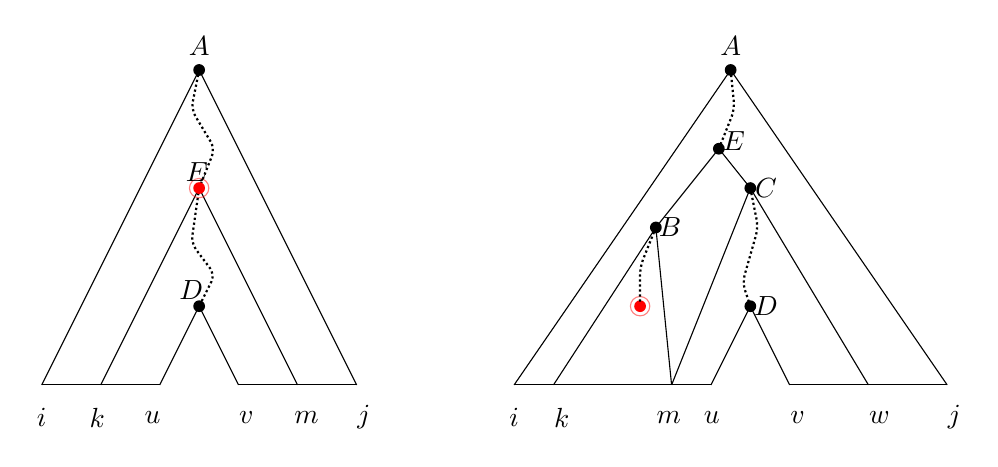
\begin{tikzpicture}
\draw (0,0) -- (1.5,0) ;
\draw (0,0) -- (2,4) ;
\draw (2,4) -- (4,0) ;
\draw (1.5,0) -- (2,1) ;
\draw (2,1) -- (2.5,0) ;
\draw (2.5,0) -- (4,0) ;
\draw (0.75,0) -- (2,2.5) ;
\draw (2,2.5) -- (3.25,0) ;
\draw [thick,densely dotted, rounded corners=1mm](2,4) --  (1.9, 3.5) -- (2.2, 3) -- (2,2.5);
\draw [thick,densely dotted, rounded corners=1mm] (2,2.5) -- (1.9, 1.8) -- (2.2, 1.4) -- (2,1);
\node (start) {}; 
\node [below=0.05cm of start] (i1) {$i$};
\node [right=3.7cm of i1] (j1) {$j$}; 
\node [right=0.3cm of i1] (k1) {$k$}; 
\node [right=1cm of i1] (u1) {$u$}; 
\node [right=2.2cm of i1] (v1) {$v$}; 
\node [right=2.9cm of i1] (m1) {$m$}; 
\node [right=2.0cm of start] (middle1) {}; 
\node (A1) at (2, 4.3) {$A$}; 
\node (D1) at (1.9, 1.2) {$D$};
\node [circle, fill=red, inner sep = 1.5pt, minimum size=1pt](cr) at (2, 2.5) {};
\draw[red, semitransparent] (2, 2.5) circle[radius=3.5pt];
\node (E1) at (1.97, 2.7) {$E$};
\node [circle, fill=black, inner sep = 1.5pt, minimum size=1pt](pD1) at (2,1) {};
\node [circle, fill=black, inner sep = 1.5pt, minimum size=1pt](pA1) at (2,4) {};

%second picture
\draw (6,0) -- (8.5,0) ;
\draw (9.5,0) -- (11.5,0) ;
\draw (6,0) -- (8.75,4) ;
\draw (8.75,4) -- (11.5,0) ;
%\draw (7,0) -- (8.8,3) ;
%\draw (8.8,3) -- (10.5,0) ;
\draw (8.5,0) -- (9,1) ;
\draw (9,1) -- (9.5,0) ;
\draw (6.5, 0) -- (7.8,2) ;
\draw (7.8,2) -- (8,0) ;
\draw (8,0) -- (9,2.5) ;
\draw (9,2.5) -- (10.5,0) ;
\draw (8.6,3) -- (9,2.5) ;
\draw (8.6,3) -- (7.8,2) ;
\node (start2) at (6, 0) {}; 
\node [below=0.05cm of start2] (i2) {$i$};
\node [right=0.2cm of i2] (k2) {$k$}; 
\node [right=1.5cm of i2] (m2) {$m$}; 
\node [right=2.1cm of i2] (u2) {$u$}; 
\node [right=3.2cm of i2] (v2) {$v$}; 
\node [right=4.2cm of i2] (w) {$w$}; 
\node [right=5.2cm of i2] (j2) {$j$}; 
\node (A2) at (8.75, 4.3) {$A$}; 
\node (E2) at (8.79, 3.1) {$E$}; 
\node (B) at (7.98, 2) {$B$}; 
\node (C) at (9.2,2.5) {$C$}; 
\node (D2) at (9.2,1) {$D$}; 
\node [circle, fill=black, inner sep = 1.5pt, minimum size=1pt](pB) at (7.8,2) {};
\node [circle, fill=red, inner sep = 1.5pt, minimum size=1pt](crU) at (7.6,1) {};
\draw[red, semitransparent] (7.6, 1) circle[radius=3.5pt];
\node [circle, fill=black, inner sep = 1.5pt, minimum size=1pt](pA2) at (8.75,4) {};
\node [circle, fill=black, inner sep = 1.5pt, minimum size=1pt](pC) at (9,2.5) {};
\node [circle, fill=black, inner sep = 1.5pt, minimum size=1pt](pE2) at (8.6,3) {};
\node [circle, fill=black, inner sep = 1.5pt, minimum size=1pt](pD2) at (9,1) {};
\draw [thick,densely dotted, rounded corners=1mm](9,2.5) -- (9.1, 2) -- (8.9, 1.3) -- (9,1) ;
\draw [thick,densely dotted, rounded corners=1mm](8.75,4) -- (8.8, 3.5) -- (8.6,3);
\draw [thick,densely dotted, rounded corners=1mm]  (7.8,2) -- (7.6, 1.5) -- (7.6,1.05);
\end{tikzpicture}
% Use the relevant command to insert your figure file.
% For example, with the graphicx package use
% figure caption is below the figure
\caption{ Cases for conditional proposition $\frac{A}{D}(i , u :: v, j)$: (left) a subtree with the critical node at the root contains the hole; (right) a subtree with the critical node at the root contains only leaves corresponding to the path $i \rightarrow u$.}
\label{proofcases}       % Give a unique label
\end{figure}



\begin{enumerate}
\item \textit{A subtree with the critical node at the root contains the hole $u :: v$.} 
\\ Let $E$ be a label of the critical node. Then a corresponding subtree splits the path from the vertex $i$ to the vertex $u$ onto two paths: $i \rightarrow k$ and $k \rightarrow u$ and the path from the vertex $v$ to the vertex $j$ onto $v \rightarrow m$ and $m \rightarrow j$ respectively (as illustrated in Figure \ref{proofcases} (left)). The next proof tree represents the proof of the proposition $\frac{A}{D}(i , u ::v, j)$ in this case. 
\begin{prooftree}
\AxiomC{$\frac{A}{E}(i , k :: m , j)$}
\AxiomC{$\frac{E}{D}(k , u :: v , m)$}
\BinaryInfC{ $\frac{A}{E}(i , u :: v , j)$}
\end{prooftree}
Conditional proposition $\frac{A}{E}(i , k :: m , j)$ and $\frac{E}{D}(k , u :: v , m)$ have no more than $\frac{2}{3}l$ leaves, so $\frac{A}{E}(i , u :: v , j)$ has a proof of logarithmic height.

\item \textit{A subtree with the critical node at the root contains only leaves corresponding to the path from the vertex $i$ to the vertex $u$ in the input graph.}


This case is illustrated in Figure \ref{proofcases} (right). Consider the biggest subtree which contains a subtree with the critical node at the root and has leaves corresponding only to the path from the vertex $i$ to the vertex $u$ of the input graph. Let $B$ be a label at the root of this tree and $k \rightarrow m$  be a corresponding path in the input graph. Let $E$ be a parent node of node $B$ and let $C$ be a second child of $E$ (for $E \rightarrow BC \in P$). A parse tree with the root labelled by $C$ has some leaves corresponding to the path $v \rightarrow j$, so let $w$ be a vertex which splits this path on two. Now we are able to write the proof of $\frac{A}{E}(i , u :: v , j)$.
\begin{prooftree}
\AxiomC{$\frac{A}{E}(i , k :: w , j)$}
\AxiomC{$B(k, m)$}
\UnaryInfC{$\frac{E}{C}(k , m :: w)$}
\AxiomC{$\frac{C}{D}(m , u :: v , w)$}
\BinaryInfC{$\frac{E}{D}(k , u ::v , w)$}
\BinaryInfC{ $\frac{A}{D}(i , u :: v , j)$}
\end{prooftree}
The subtree with the root labelled $B$ obviously contains at least $\frac{2}{3}l$ leaves, so each of the other propositions $\frac{C}{D}(m , u :: v , w)$ and $\frac{A}{E}(i , k :: w , j)$ has no more then  $\frac{2}{3}l$ leaves. By induction hypothesis they have a proof of logarithmic height. Thus, proposition  $\frac{A}{D}(i , u :: v , j)$ can be proved via 4 steps using propositions with the proofs of logarithmic depth.
\\The case when the subtree with the critical node at the root contains only leaves corresponding to the path from the vertex $v$ to the vertex $j$ in the input graph is held symmetrically.
\end{enumerate}
Before we will make a conclusion, the following definition should be introduced.
\begin{definition}
\label{L}
Let $G = (\Sigma, N, P)$ be a context-free grammar and $D$ be a directed labelled graph. Then $\mathzapf{L}$ is the length of longest shortest path $i \pi j$ for all triples $(A, i, j)$, where $j$ is reachable from $i$ via path labelled by $l(i\pi j) \in L(G_A)$ and $A \in N$.
\end{definition}
\end{proof}
Using lemmas above, we can conclude the following.
\begin{corollary}
\label{coldepth}
Let $G = (\Sigma, N, P)$ be a context-free grammar in Chomky normal form and let $\mathzapf{L}$ be the length of the maximum in all nonterminals and all pairs of graph nodes shortest path labelled by a string from $L(G)$ (see Definition \ref{L}). Then there is a uniform family of circuits for solving CFL-reachability problem on the graphs with $n$ nodes, which are of depth $O(\log n \log \mathzapf{L})$ and contain $O(n^6)$ elements.
\end{corollary}


The depth and therefore the efficiency of the circuit depends on the value of parameter $\mathzapf{L}$. We investigate bounds for $\mathzapf{L}$ in the next two sections.

\section{Efficient subclasses of context-free languages}
\label{sec:CF}
In this section our focus is on estimating the value of $\mathzapf{L}$ for some fixed context-free languages and arbitrary input graphs. 
\subsection{General case}
Hellings in \cite{HellingsCFPQ} gave the worst-case lower and upper bounds on the $\mathzapf{L}$ parameter.
\begin{theorem}[Hellings]
Let  $G = (\Sigma, N, P)$ be a context-free grammar and $D=(V, E, \Sigma)$ be a directed labelled graph with $n$ nodes. In the worst case, we have $ n^22^{|N|}\le \mathzapf{L} \le 2^{|N|n^2-1}$.
\end{theorem}


Using the bounds above and Corollary \ref{coldepth}, we can get the maximum depth of our circuit in the worst case: 
$O(\log n \log \mathzapf{L}) = O(\log n \log 2^{|N|n^2-1}) = \\ = O(|N|n^2\log n)$. The circuit can have a depth which is polynomial on the input length in case of arbitrary context-free grammar. It is not surprising because of the nature of P-completeness: we don't have an efficient parallel algorithm or circuit with a polylogarithmic on the input length depth for CFL-reachability problem because it is P-complete problem (unless $P \neq NC$).


But we also have a polynomial lower bound on $\mathzapf{L}$, which give us the effective circuit with depth $O(\log^2 n)$ in some cases. Our next goal is to investigate important subclasses of context-free languages, and find those for which CFL-reachability is in the class $NC$.
\subsection{Rational index}
It is known that the value of $\mathzapf{L}$ is different for various types of context-free languages, in particular it can be bounded from above by the polynomial or exponential function on the number of graph nodes \cite*{Dyck1, CFRat, GreibRat}. Boasson et al. in \cite{RatBasic} introduced definition of such function called \textit{rational index}. For a language $L$ over an alphabet $\Sigma$, its rational index $\rho_L$ is a function defined as follows:
\begin{equation}
\rho_L(n) = \max\{\min\{|w|:w \in L \cap K\}, K \in {Rat}_n, L \cap K \neq \emptyset\},
\end{equation} where $|w|$ is the length of a word $w$ and ${Rat}_n$ denotes the set of regular languages on an alphabet $\Sigma$, recognized by a finite nondeterministic automation with at most $n$ states.


It is easy to see that in the case of fixed context-free language and arbitrary graph, $\mathzapf{L}$ is some kind of the rational index: we can represent arbitrary graphs with $n$ nodes via nondeterministic automations with at most $n$ states, then $\mathzapf{L}$ is exactly rational index. So, we have the following corollary.
\begin{corollary}
\label{ratdepth}
Let $L$ be a context-free language on an alphabet $\Sigma$, which has a polynomially bounded from above rational index, and $D=(V, E, \Sigma)$ be a directed labelled graph with $n$ nodes. Then, CFL-reachability problem for $L$ and $D$ is in $NC^2$.
\end{corollary}


For example, language $L = \{a^nb^m, n \neq m\}$ has polynomial rational index $\rho_L(n) = 2n -1$ \cite{GreibRat}, so CFL-reachability problem for $L$ and arbitrary directed labelled graph with $n$ nodes is in $NC^2$.
\subsection{Linear, metalinear and superlinear languages}
A \textit{linear language} is a language generated by some \textit{linear grammar}. A \textit{linear grammar} is a context-free grammar that has at most one nonterminal in the right hand side of each of its productions. The linear grammar  $G = (\Sigma, N, P)$ is said to be in the Chomsky normal form, when all of its production rules are of the form: $A \rightarrow aB$, or $A \rightarrow Ba$, or $A \rightarrow a$, where $B \in N$ and $a \in \Sigma$.


Before we consider the value of $\mathzapf{L}$ for linear grammars, we shall prove the following.
\begin{lemma}
\label{lem:treeheight}
Let  $G = (\Sigma, N, P)$ be a context-free grammar,  $D=(V, E, \Sigma)$ be a directed labelled graph with $n$ nodes and $\pi$ be the maximum in all nonterminals and all pairs of graph nodes shortest path labelled by a string from $L(G)$. Then a height of a parse tree for $l(\pi)$ does not exceed $|N|n^2$.
\end{lemma}

\begin{proof}
 Assume that the parse tree for $l(\pi)$ has a height of more than $|N|n^2$. There are $|N|n^2$ unique labels $(A, i, j)$ for nodes of the parse tree, so according to the pigeonhole principle, the parse tree for $l(\pi)$ contains at least one subtree $T$ with label $(A, i, j)$ at the root, which has a subtree $T'$ with the same label. Then we can change $T$ with $T'$ and get a new string $l(\pi')$ which is shorter than $l(\pi)$. But $l(\pi)$ is the shortest, then we have a contradiction.

\end{proof}
\begin{theorem}
\label{thlin}
Let  $G = (\Sigma, N, P)$ be a linear grammar and $D=(V, E, \Sigma)$ be a directed labelled graph with $n$ nodes. Then the length of the maximum in all nonterminals and all pairs of graph nodes shortest path labelled by a string from $L(G)$ ($\mathzapf{L}$) is $O(|N|n^2)$.
\end{theorem}

\begin{proof}
From Lemma \ref{lem:treeheight}, a height of a parse tree is no more then $|N|n^2$. Let's construct a parse tree of such height for linear grammar in the Chomsky normal form. Every rule for linear grammar has at most one nonterminal in the right hand side of each of its productions, so if the grammar is in the Chomsky normal form, then there is the only one terminal symbol at the every level of the parse tree (as illustrated in Figure \ref{ptlin} (left)). The tree has no more then $|N|n^2$ levels, so the length of any shortest path labelled by a string from $L(G)$ is no more than $O(|N|n^2)$.
\end{proof}
\begin{figure}
\begin{tikzpicture}
\node{S}
 child {node {$A$} 
      child {node {$b$}}
      child { node {$B$}
        child { node {$c$}}
        child { node {$C$}
                     child {node {$...$}}
                     child { node {$d$}} }
         }
     }
     child {node {$a$}};
\end{tikzpicture}
\begin{tikzpicture}[level 1/.style={sibling distance=18mm}, level 2/.style={sibling distance=8mm},  level 3/.style={sibling distance=8mm}]
\node{S}
 child {node {$A_1$}
     child {node {$\alpha \in \Sigma^*$}} 
     child {node {$A_{i}$}
           child {node {$\gamma \in \Sigma^*$}} 
           child {node {$A_{j}$}
                       child {node {$...$}} 
           } 
           child {node {$\theta \in \Sigma^*$}} 
     } 
    child {node {$\beta \in \Sigma^*$}} 
}
child {node {$A_2$}
    child {node {$...$}} 
}
child {node {$A_3$}
    child {node {$...$}} 
}
 child {node {$A_4$} 
      child {node {$\theta \in \Sigma^*$}}
      child { node {$A_j$}
        child { node {$...$} }
        }
        child { node {$\alpha \in \Sigma^*$}} 
     };
\end{tikzpicture}
% Use the relevant command to insert your figure file.
% For example, with the graphicx package use
% figure caption is below the figure
\caption{A parse tree for linear grammar in the Chomsky normal form (left) and for metalinear grammar with width $m=4$ (right).}
\label{ptlin}       % Give a unique label
\end{figure}


Combining Theorem \ref{thlin} and Corollary \ref{coldepth} we are able to conclude the following.
\begin{corollary} 
\label{linear}
Let  $G = (\Sigma, N, P)$ be a linear grammar and $D=(V, E, \Sigma)$ be a directed labelled graph with $n$ nodes. Then CFL-reachability problem for $G$ and $D$ is in $NC^2$.
\end{corollary}


There are natural extensions of linear languages: \textit{metalinear} and \textit{superlinear} languages. Just like linear languages, these classes of context-free languages are known to be easy to parse \cite{Jayaram2017ApproximatingLE}. We will show that they are ``easy`` for our circuit too.


\paragraph{Metalinear languages}

Let $G = (\Sigma, N, P, S)$ be a context-free grammar. $G$ is \textit{meatalinear} if all productions of $P$ are of the following forms:
\begin{enumerate}
\item $S \rightarrow A_1A_2...A_m$, where $A_i \in N - \{S\}$
\item $A \rightarrow u$, where $A \in N - \{S\}$ and $u \in (\Sigma^*((N-\{S\}) \cup {\varepsilon})\Sigma^*)$
\end{enumerate}


The width of a metalinear grammar is $max\{m$ | $S \rightarrow A_1A_2...A_m \}$. Metalinear languages of width 1 are obviously linear languages.
\begin{lemma}
\label{thmetalin}
Let  $G = (\Sigma, N, P)$ be a metalinear grammar, where $G_S$ has the width $m$, $k$ be a length of the longest sequence of terminal symbols in the right-hand-side of rules and $D=(V, E, \Sigma)$ be a directed labelled graph with $n$ nodes. Then the length of the maximum in all nonterminals and all pairs of graph nodes shortest path labelled by a string from $L(G)$ ($\mathzapf{L}$) is $O(mk|N|n^2)$.
\end{lemma}
\begin{proof}
Consider the highest parse tree for metalinear grammar. By Lemma \ref{lem:treeheight}, it's height is no more then $|N|n^2$. Obviously, if the root of the tree is labelled by some $A_i  \in N - \{S\}$, value of $\mathzapf{L}$ in this case is the same as value of $\mathzapf{L}$ for the case of linear grammar --- $O(|N|n^2)$ for constant value of $k$. If the root of the tree is labelled by $S$, the tree looks like as illustrated in Figure \ref{ptlin} (right). It is easy to see that there are no more than $km$ terminal symbols on every level of such tree. Thus, we have $\mathzapf{L}$ = $O(mk|N|n^2)$. 
\end{proof}
\begin{figure}
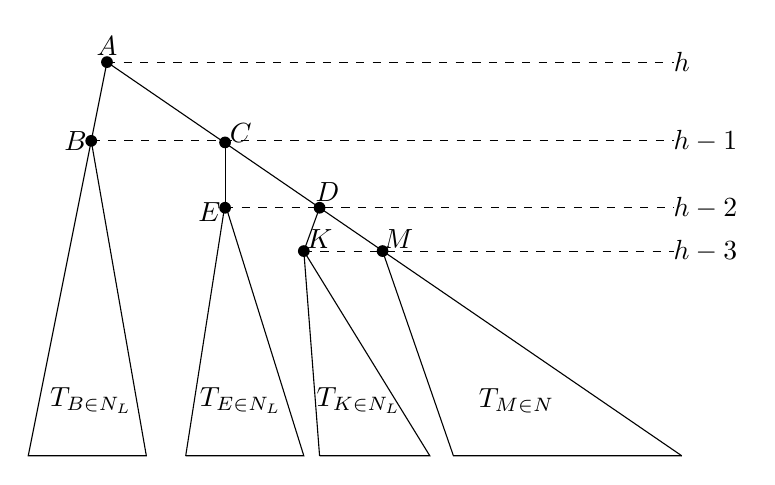
\begin{tikzpicture}

\draw(1.8,5.3) -- (9.1,0.3) ;
\draw(1.8,5.3) -- (0.8,0.3) -- (2.3,0.3) -- (1.6,4.3);
\draw (2.8,0.3) -- (4.3,0.3) -- (3.3, 3.5) -- (2.8,0.3);
\draw (4.5,0.3) -- (5.9,0.3) -- (4.3, 2.9) -- (4.5,0.3);
\draw (3.3, 3.5) -- (3.3, 4.28);
\draw (4.3, 2.9) -- (4.5, 3.45);
\draw  (9.1,0.3) -- (6.2,0.3) --  (5.3, 2.9);

\draw[dashed](1.8,5.3) -- (9,5.3) ;
\draw[dashed] (1.6,4.3) -- (9,4.3);
\draw[dashed] (3.3, 3.45) -- (9,3.45);
\draw[dashed] (4.3, 2.9) --  (9,2.9) ;

\node at (9.1,5.3) {$h$};
\node at (9.4,4.3) {$h-1$};
\node at (9.4,3.45) {$h-2$};
\node at (9.4,2.9) {$h-3$};

\node [circle, fill=black, inner sep = 1.5pt, minimum size=1pt] at (1.8,5.3) {};
\node [circle, fill=black, inner sep = 1.5pt, minimum size=1pt] at (1.6,4.3) {};
\node [circle, fill=black, inner sep = 1.5pt, minimum size=1pt] at (3.3, 4.28) {};
\node [circle, fill=black, inner sep = 1.5pt, minimum size=1pt] at (3.3, 3.45) {};
\node [circle, fill=black, inner sep = 1.5pt, minimum size=1pt] at (4.5, 3.45) {};
\node [circle, fill=black, inner sep = 1.5pt, minimum size=1pt] at (4.3, 2.9) {};
\node [circle, fill=black, inner sep = 1.5pt, minimum size=1pt] at (5.3, 2.9) {};

\node (start) at (1.8, 5.5) {$A$}; 
\node (first) at (1.4, 4.3) {$B$}; 
\node (firstr) at (3.5, 4.4) {$C$}; 
\node (second) at (3.1, 3.4) {$E$}; 
\node (secondr) at (4.6, 3.65) {$D$}; 
\node (third) at (4.5, 3.05) {$K$}; 
\node (thirdr) at (5.5, 3.05) {$M$}; 
\node (firstt) at (1.6, 1) {$T_{B \in N_L}$}; 
\node (firstt) at (3.5, 1) {$T_{E \in N_L}$}; 
\node (firstt) at (5, 1) {$T_{K \in N_L}$}; 
\node (firstt) at (7, 1) {$T_{M \in N}$}; 
\end{tikzpicture}
% Use the relevant command to insert your figure file.
% For example, with the graphicx package use
% figure caption is below the figure
\caption{A worst-case parse tree for superlinear grammar.}
\label{superlin}       % Give a unique label
\end{figure}

Applying Lemma \ref{thmetalin} and Corollary \ref{coldepth}, we deduce with the corollary.
\begin{corollary} 
Let  $G = (\Sigma, N, P)$ be a metalinear grammar and $D=(V, E, \Sigma)$ be a directed labelled graph with $n$ nodes. Then CFL-reachability problem for $G$ and $D$ is in $NC^2$.
\end{corollary}
\paragraph{Superlinear languages}
Let $G = (\Sigma, N, P)$ be a context-free grammar. $G$ is \textit{superlinear} if all productions of $P$ satisfy these conditions:
\begin{enumerate}
\item there is a subset $N_L \subseteq N$ such that every $A \in N_L$ has only linear productions $A\rightarrow aB$ or $A\rightarrow Ba$, where $B \in N_L$ and $a \in \Sigma$.
\item if $A \in N \setminus N_L$, then $A$ can have non-linear productions of the form $A \rightarrow BC$ where $B\in N_L$ and $C \in N$, or linear productions of the form $A\rightarrow \alpha B$ | $B \alpha$ | $\alpha$ for $B \in N_L$, $\alpha \in \Sigma^*$.
\end{enumerate}


It can be seen from conditions above, that superlinear grammars contain the metalinear grammars.
\begin{lemma}
\label{superlin}
Let  $G = (\Sigma, N, P)$ be a superlinear grammar and $D=(V, E, \Sigma)$ be a directed labelled graph with $n$ nodes. Then the length of the maximum in all nonterminals and all pairs of graph nodes shortest path labelled by a string from $L(G)$ ($\mathzapf{L}$) is $O(|N^2|n^4)$.
\end{lemma}
\begin{proof}
Let's construct a parse tree of maximum height $h$ from the root to leaves. Let $A$ be a nonterminal at the root of the parse tree $T_A$. We have two cases to consider:
\begin{enumerate}
\item  $A \in N_L$ or $A \in N \setminus N_L$ and $A$ has linear productions: then the tree with $A$ at the root is the same tree as parse tree for linear grammar and it has $O(h)$ leaves.
\item  $A \in N \setminus N_L$ and $A \rightarrow BC \in P$: then number of leaves in the tree $le(T_A)$ can be expressed with the following reccurent formula: $le(T_A) = le(T_B) + le(T_C) = h(T_B) + le(T_C) = h(T_A) - 1 + le(T_C)$.
\end{enumerate}
In the worst case, we have to add tree with $i$ leaves on every $i$-th level of the parse tree (counting from $h-1$ to 0) (see Figure \ref{superlin}). By Lemma  \ref{lem:treeheight}, $h \le |N|n^2$, so in the worst case the highest tree will have $|N|n^2-1 + |N|n^2 - 2 ... + 1 = O(|N^2|n^4)$ leaves.
\end{proof}


Combining Lemma \ref{superlin} and Corollary \ref{coldepth} we are able to conclude the following.
\begin{corollary} 
Let  $G = (\Sigma, N, P)$ be a superlinear grammar and $D=(V, E, \Sigma)$ be a directed labelled graph with $n$ nodes. Then CFL-reachability problem for $G$ and $D$ is in $NC^2$.
\end{corollary}

\subsection{Dyck languages}
\textit{Dyck language over $\Sigma_k$} is the set of well-balanced words over alphabet $\Sigma_k = \{(_1, (_2, ..., (_k, )_1, )_2, ..., )_k\}$. Dyck language can be defined by the following rules:
\\$S \rightarrow SS$ | $S \rightarrow \varepsilon$ |$S \rightarrow (_1S)_1$ | $S \rightarrow (_2S)_2$ | ... | $S \rightarrow (_kS)_k$, where $S$ is the start symbol, and $\varepsilon$ is the empty string. We will denote the Dyck language over $\Sigma_i$ by $D_i$.


Dyck languages play an important role in formal languages theory. The famous Chomsky-Sch\"utzenberger theorem states that every context-free language $L$ can be represented via a regular language $R$ and a Dyck language $D_n$, which are combined by means of an intersection and a homomorphism $h$. 
\begin{equation}
L = h(D_n \cap R)
\end{equation}


Because every context-free language can be represented with Dyck language, it is natural to expect that CFL-reachability is P-complete for Dyck languages. P-completeness for the similiar problem LGAP in case of $D_2$ was proved in \cite*{PCompl, LReach, Regularrealizability}. We will show that $\mathzapf{L}$ is exponential for $D_k$ where $k\ge2$, so our circuit is not effective in that case.
\begin{lemma}[Pierre]
\label{pierrelem}
The rational indexes of generators of context-free languages belongs to $exp(\Theta(n^2/\ln n))$.
\end{lemma}
\begin{theorem}
Let $L$ be a Dyck language over $k \ge 2$ brackets and $D=(V, E, \Sigma)$ be a directed labelled graph with $n$ nodes. Then, $\mathzapf{L}$  belongs to $exp(\Theta(n^2/\ln n))$.
\end{theorem}
\begin{proof}
By definition, generator is a context-free language which can transform into any context-free language through a rational transduction \cite{CFRat}.
Notice that for $k>2$ there is a homomorphism $g$ such that $D_k = g^{-1}(D_2)$ can be constructed. Thanks to the Chomsky-Sch\"utzenberger theorem, we have the following equation.
\begin{equation}
L = h(g^{-1}(D_2)\cap R)
\end{equation}
Thus, every context-free language can be generated by $D_k$, where $k \ge 2$. By \ref{pierrelem} we can conclude that $\mathzapf{L}$ for $D_k$ belongs to $exp(\Theta(n^2/\ln n))$. 
\end{proof}


We remark that strict upper bound on $\mathzapf{L}$ for arbitrary context-free grammar is obtained from Lemma \ref{pierrelem}, so it answers to the corresponding open question stated in \cite{HellingsCFPQ}.


It is known that $D_1$ is a generator of \textit{one-counter languages} \cite{GreibHier}. \textit{One-counter} languages are the languages recognized by \textit{one-counter automata} --- pushdown automata with a single stack symbol. For example, $L = \{w\#w'$ | $|w| \neq |w'|\}$ is one-counter language.



\begin{lemma}[Deleage, Pierre]
\label{dyck1lem}
The rational index of $D_1$ is in $O(n^2)$.
\end{lemma}
\begin{theorem}
\label{onecounter}
Let $L$ be a one-counter language, and $D=(V, E, \Sigma)$ be a directed labelled graph with $n$ nodes. Then, CFL-reachability problem for $L$ and $D$ is in $NC^2$.
\end{theorem}
\begin{proof} 
Because $D_1$ is a generator of one-counter languages \cite{GreibHier}, $D_1$ rationally dominates any one-counter language. If $L$ rationally dominates $L'$, then there exists an integer $c$ such that for every $n \in \mathbb{N}$ $\rho_{L'(n)} < cn(\rho_L(cn) + 1)$ \cite{RatBasic}.  Thus, the rational index of any one-counter language doesn't exceed $O(n^3)$, and by Corollary \ref{coldepth}, the depth of the circuit for one-counter languages is $O(\log^2 n)$.
\end{proof}


Notice that there is an effective sequential algorithm for CFL-reachability for $D_1$ based on matrix multiplication \cite{Bradford}. We believe that using Theorem \ref{onecounter} it can be extended for working with one-counter languages.

\subsection{Greibach languages and substitution closures}
\begin{figure}
\centering
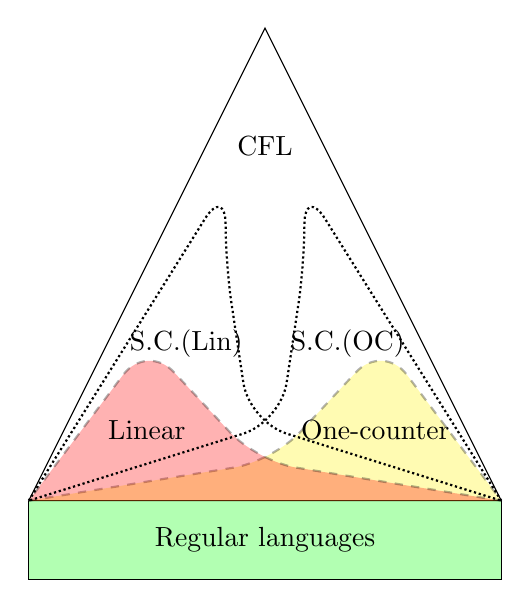
\begin{tikzpicture}
\draw[fill=green, opacity=0.3](0,1) -- (0,0) -- (6,0) --  (6,1);
\draw(0,1) -- (0,0) -- (6,0) --  (6,1);
\draw(0,1) -- (6,1) -- (3, 7) -- (0,1) ;
\draw[thick, dashed, rounded corners=5mm, fill=yellow, opacity=0.3] (0,1) -- (3.1, 1.5) -- (4.5, 3) -- (6,1);
\draw[thick, dashed, rounded corners=5mm, fill=red, opacity=0.3] (6,1) -- (2.9, 1.5) -- (1.5, 3) -- (0,1);
\draw[thick, densely dotted, rounded corners=5mm](0,1) -- (2.5, 5) -- (2.5,4)-- (2.8, 2) -- (6,1);
\draw[thick, densely dotted, rounded corners=5mm](6,1) -- (3.5, 5) -- (3.5,4)-- (3.2, 2) -- (0,1);
\node (reg) at (3, 0.5) {Regular languages}; 
\node (cfl) at (3, 5.5) {CFL}; 
\node (lin) at (1.5, 1.9) {Linear}; 
\node (one) at (4.4, 1.9) {One-counter}; 
\node (linsc) at (2, 3) {S.C.(Lin)}; 
\node (ocsc) at (4.05, 3) {S.C.(OC)}; 
\end{tikzpicture}
\caption{A hierarchy of linear languages (Lin), one-counter languages (OC) and their substitution closures (S.C).}
\label{hierarchy}      
\end{figure}
Consider families of linear and one-counter languages. We can see that they are ``easy'' for CFL-reachability (Theorem \ref{onecounter}, Corollary \ref{linear}). One reason for this is that they are defined by natural restrictions on grammars or pushdown automatons (PDA). Restricting a PDA such that the height of its stack is only allowed to increase and then to decrease, thus performing only one turn, leads to the definition of one-turn PDAs. It is known that these PDAs can be characterized by linear grammars \cite{KUTRIB20072152}. One-counter languages are recognized by PDA with only one stack symbol. The same restrictions holds for substition closures of these languages, because substitution corresponds to a nesting of the pushdown stack \cite{Ginsburg1975}. It is easily observed that substitution closure of polinomially-bounded $\mathzapf{L}$ language yields polinomially-bounded $\mathzapf{L}$ language. 


But some of the restrictions on the pushdown store or on the grammar cannot be simulated by others. It is exactly the case of linear and one-counter languages: they and their iterated substitution closures are distinct families of context-free languages \cite{BEAUQUIER198191}.
Hierarchy of linear languages, one-counter languages and their substitution closures is illustrated in Figure \ref{hierarchy}. 


Family of \textit{Greibach languages} is the substitution closure of linear and one-counter languages. It is a large strict subfamily of the family of context-free languages: it does not contain the language $D_2$ \cite{Autebert1997}. Because it is the substitution closure of two polinomially-bounded $\mathzapf{L}$ languages, we have the following corollary.
\begin{corollary} 
Let  $L$ be a Greibach language and $D=(V, E, \Sigma)$ be a directed labelled graph with $n$ nodes. Then CFL-reachability problem for $L$ and $D$ is in $NC^2$.
\end{corollary}
\subsection{Oscillation-bounded languages}
Oscillation-bounded languages were introduced in \cite{BoundOsc}. Just like one-counter and linear languages, it is defined by restriction on the pushdown automata. This restriction is based on the notion of \textit{oscillation}, a special measure of how variable is the stack height over time. Oscillation is defined using a hierarchy of \textit{harmonics}. Let $\bar{a}$ be a \textit{push}-move and $a$ be a \textit{pop}-move. Then PDA run can be described by well-nested word of $\bar{a}$-s and $a$-s. Order 1 harmonic $h_1$ is $\bar{a}a$ $\bar{a}a$ (\textit{push pop push pop}), order 2 harmonic $h_2$ is $\bar{a}$ <order 1 harmonic> $a$ $\bar{a}$ <order 1 harmonic> $a$, so $(i+1)$-st harmonic is $\bar{a}$ $h_i$ $a$ $\bar{a}$ $h_i$ $a$.


PDA run $r$ is \textit{k-oscillating} if the harmonic of order $k$ is the greatest harmonic that is contained in $r$. \textit{Oscillation-bounded languages} are languages accepted by pushdown automata restricted to k-oscillating runs.
\begin{example}
Consider Figure \ref{oscb}. It shows how the stack height changes during the run of PDA. Corresponding well-nested word is $\bar{a}$ $\bar{a}$ $\bar{a}a$ $\bar{a}a$ $a$ $\bar{a}a$ $a$. The greatest harmonic in this word is 1 order harmonic: $\mathbf{\bar{a}}$ $\bar{a}$ $\mathbf{\bar{a}a}$ $\mathbf{\bar{a}a}$ $a$ $\bar{a}a$ $\mathbf{a}$, therefore oscillation of the run is 1.
\end{example}
\begin{figure}
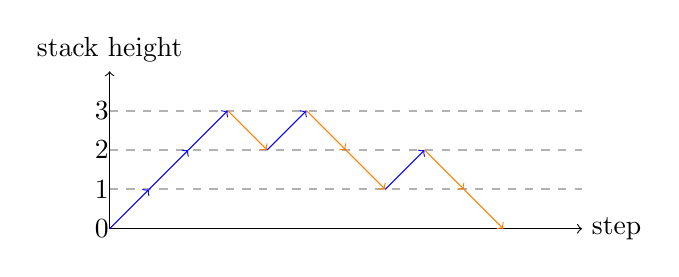
\begin{tikzpicture}
    \draw[thick, dashed, opacity=0.3] (0,0.5) -- (6,0.5);
     \draw[thick, dashed, opacity=0.3] (0,1) -- (6,1);
      \draw[thick, dashed, opacity=0.3] (0,1.5) -- (6,1.5);
      \draw[->] (0,0) -- (6,0) node[right] {step};
      \draw[->] (0,0) -- (0,2) node[above] {stack height};
     \draw[->, blue] (0,0) -- (0.5,0.5);
      \draw[->, blue] (0.5,0.5) -- (1,1);
      \draw[->, blue] (1,1) -- (1.5,1.5);
       \draw[->, orange] (1.5,1.5) -- (2,1);
    \draw[->, blue] (2,1) -- (2.5,1.5);
\draw[->, orange] (2.5,1.5) -- (3,1);
\draw[->, orange] (3,1) -- (3.5,0.5);
    \draw[->, blue]  (3.5,0.5) -- (4,1);
\draw[->, orange] (4,1) -- (4.5,0.5);
\draw[->, orange] (4.5,0.5) -- (5,0);

\node (null) at (-0.1, 0) {0}; 
\node (one) at (-0.1, 0.5) {1}; 
\node (two) at (-0.1, 1) {2}; 
\node (three) at (-0.1, 1.5) {3}; 
    \end{tikzpicture}
\caption{Stack heights during the run of PDA.}
\label{oscb}
\end{figure}


Oscillation of the run is closely related with the $dimension$ of the corresponding parse tree. For each node $v$ in a tree $T$ a dimension $dim(v)$ is inductively defined as follows:
\begin{itemize}
\item If $v$ is a leaf, then $dim(v)$ = 0
\item If $v$ is an internal node with $k$ children $v_1, v_2, ..., v_k$ for $k \ge 1$, then 
\begin{equation}
dim(v) = 
 \begin{cases}
   \max_{i \in \{1...k\}}dim(v_i) &\text{if there is a unique maximum}\\
   \max_{i \in \{1...k\}}dim(v_i)+1 &\text{otherwise}
 \end{cases}
\end{equation}
\end{itemize}


Dimension of a parse tree $T$ $dim(T)$ is a dimention of it's root.  It is observable from the definition that dimension of a tree $T$ is the height of the largest perfect binary tree, which can be obtained from $T$ by contracting edges and accordingly identifying vertices. A tree with dimension $dim(T) = 2$ is illustrated in Figure \ref{oscbtree}.


It is known that the dimension of parse trees and the oscillation defined on PDA runs are in linear relationship.
\begin{figure}
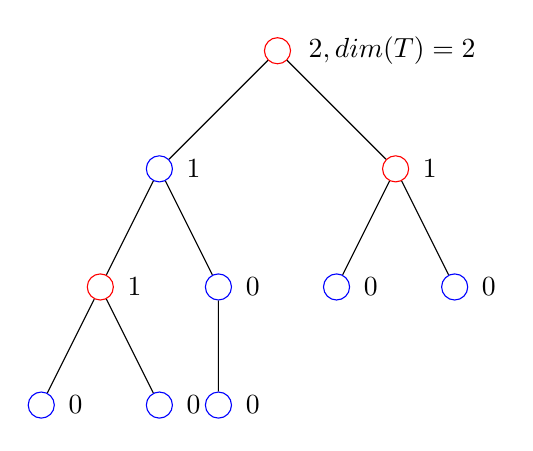
\begin{tikzpicture}[
level 1/.style={sibling distance=3cm},
level 2/.style={sibling distance=1.5cm}]
%\tikzstyle{every node}=[circle,draw]

\node[circle,draw] (Root) [red] {}
    child {
    node[circle,draw, blue] (l) {} 
    child { node[circle,draw, red](ll) {}
            child { node[circle,draw, blue] (p) {} }
            child { node[circle,draw, blue] (pl) {} }
             }
    child { node[circle,draw, blue](lr) {} 
          child { node[circle,draw, blue] (plr) {} }
      }
}
child {
    node[circle,draw, red] (r) {}
    child { node[circle,draw, blue] (rl) {}} 
    child { node[circle,draw, blue] (rr) {} }
};
\node  [right=0.05cm of p] {0};
\node  [right=0.1cm of Root] {$2, dim(T)=2$};
\node  [right=0.05cm of l] {1};
\node  [right=0.05cm of r] {1};
\node  [right=0.05cm of ll] {1};
\node  [right=0.05cm of lr] {0};
\node  [right=0.05cm of pl] {0};
\node  [right=0.05cm of plr] {0};
\node  [right=0.05cm of rl] {0};
\node  [right=0.05cm of rr] {0};
\end{tikzpicture}
\caption{A tree $T$ with $dim(T)=2$.}
\label{oscbtree}            
\end{figure}
\begin{lemma}[Ganty, Valput]
Let a grammar $G = (\Sigma, N, P)$ be in Chomsky normal form and let $T$ be a parse tree of $G$. We have that $osc(T) - 1 \le dim(T) \le 2osc(T)$.
\end{lemma}

It is not hard to see that if $L(G)$ is $k$-oscillation-bounded language, parse trees of $G$ always have a bounded dimension.
\begin{lemma}
\label{oscbnddim}
Let $L$ be a $k$-oscillation-bounded language with grammar $G = (\Sigma, N, P)$ in Chomsky normal form and $D=(V, E, \Sigma)$ be a directed labelled graph with $n$ nodes. Then the length of the maximum in all nonterminals and all pairs of graph nodes shortest path labelled by a string from $L(G)$ ($\mathzapf{L}$) is no more than $O((|N|n^2)^{k/2})$.
\end{lemma}
\begin{proof}
Proof by induction on dimension $dim(T)$ (if oscillation is bounded by $k$, then dimension value is at most $2k$).
\\
\textbf{Basis.} $dim = 1$.
\\
Consider the worst-case tree $T$ with the dimension $dim(T) = 1$. The root of the tree has the same dimension and has two children (because the grammar in Chomsky normal form). There are two cases:  first, when both of child nodes have dimension equal to 0, then the tree has only two leaves and second, when one of children has a dimension 1, and the second child has a dimension equal to 0. For the second case we can recursively construct a tree of maximum height $|N|n^2$ (Lemma \ref{lem:treeheight}). Every internal node of such tree has two children, one of wich has dimension equal to 0 and therefore has only one leaf. This tree is exactly the worst-case tree for linear grammar in Chomsky normal form, so the number of leaves in such tree is $O(h) = O(|N|n^2)$, where $h$ is the height of the tree. Thanks to Lemma \ref{oscbnddim}, the maximum value of oscillation for $dim(T) = 1$ is 2, so $\mathzapf{L}$ is no more than $O(h^{k/2}) = O((|N|n^2)^{k/2}) = O(|N|n^2)$.
\\
\textbf{Inductive step.} $dim = d + 1$.
\\
Assume $\mathzapf{L}$ is no more than $O(h^{d})$ for every $d$, where $h$ is the height of the tree. We have two cases for the root node with dimension equal to $d+1$: 1) both of children have a dimension equal to $d$, then by proposition the tree of heght $h$ has no more than $O(h^{d})$ leaves; 2) one of children has a dimension $d + 1$, and the second child $v$ has a dimension $dim(v) \le d$. Again, a tree of maximum height with the maximum number of leaves can be constructed recursively:  each node of such tree has two children $u$ and $v$ with dimension $d+1$ and $d$ respectively (the more value of dimension of the node, the more leaves in the corresponding tree). By proposition we have no more than $(h-1)^d + (h-2)^d + (h-3)^d + ... + 1 = O(h^{d+1})$ leaves, so proposition holds for $dim = d+1$. Finally, we have $\mathzapf{L}$ is no more than $O(h^{d}) = O((|N|n^2)^{k/2})$ for every $k$.
\end{proof}


As we can see from the proof above, the family of linear languages is included in the family of oscillation-bounded languages. The reason is that the family of oscillation-bounded languages generalizes the family of languages accepted by finite-turn pushdown automata \cite{BoundOsc}. It is interesting that for arbitrary CFL, particularly for $D_2$ , the value of osciilation is not constant-bounded: it depends on the length of input and does not exeed $O(\log n)$ for the input of length $n$ \cite*{Wechsung, Gundermann}.


Combining Lemma \ref{oscbnddim} and Corollary \ref{coldepth}, we have the following.
\begin{corollary} 
Let  $L$ be a $k$-oscillation-bounded language and $D=(V, E, \Sigma)$ be a directed labelled graph with $n$ nodes. Then CFL-reachability problem for $L$ and $D$ is in $NC^2$.
\end{corollary}



\subsection{LL(k) languages and a determinism}
LL(k) languages represent another kind of restriction: unlike previous cases, which describe restrictions on PDA, \textit{LL(k) grammars} have constraints for their productions.


For a natural number $k \ge 0$, a context-free grammar $G = (\Sigma, N, P)$ is an \textit{LL(k) grammar} if for each terminal symbol string $w \in \Sigma^*$ of length up to $k$, for each nonterminal symbol $A \in V$, and for each terminal symbol string $w_{1}\in \Sigma ^{*}$ there is at most one production rule $p \in P$ such that for some terminal symbol strings $w_{2},w_{3}\in \Sigma ^{*}$ the following conditions hold:
\begin{itemize}
\item the string $w_{1}Aw_{3}$ can be derived from the start symbol $A \in N$,
\item  $w_{2}$ can be derived from $A$ after first applying rule $p$,
\item the first $k$ symbols of $w$ and of $w_{2}w_{3}$ agree.
\end{itemize}


LL(k) languages are connected with \textit{simple deterministic languages}. A context-free grammar $G = (\Sigma, N, P)$ is simple if it is in Greibach normal form and if, for each pair $(A, \alpha) \in N \time \Sigma$, there is at most one rule of the form $A \rightarrow \alpha Y_1 Y_2 ... Y_n$. A language is simple deterministic if it can be generated by a simple grammar. Simple deterministic languages are included in the family of LL(1) languages. It is known that $D_n$ is simple deterministic language \cite{SDet}, so we have exponential value of $\mathzapf{L}$ for LL(k) languages in the worst case (because LL(0) $\subsetneq$ LL(1)  $\subsetneq$ LL(2)  $\subsetneq$ ...  $\subsetneq$ LL(k)). Example \ref{exll} shows how an advantage of having the unique production is lost in case of graph input even for LL(1) grammars.
\begin{figure}
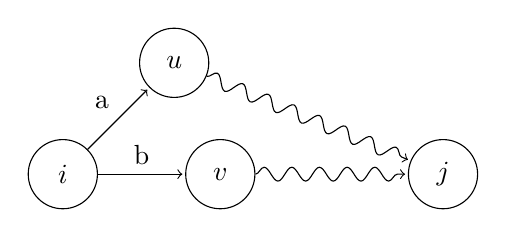
\begin{tikzpicture}[shorten >=1pt,node distance=2cm,on grid,auto] 
   \node[state] (i)   {$i$}; 
     \node[state] (u) [above right=of i ]  {$u$}; 
     \node[state] (v) [right=of i]  {$v$}; 
   \node[state] (j) [below right=of u, xshift=2cm]   {$j$}; 
    \path[->]          
    (i) edge node {a} (u)
    (i) edge node {b} (v)
    (u) edge[decorate, decoration={snake}]  node {} (j)
    (v) edge[decorate, decoration={snake}] node {} (j);
\end{tikzpicture}
\\
	\caption{A labelled graph with distinct paths from $i$ to $j$.}
\label{graphll}
\end{figure}
\begin{example}
\label{exll}
Let $G = (\Sigma, N, P)$ be a LL(1) grammar with rules $p_1$:$A \rightarrow a X_1... X_k$ and $p_2:$$B \rightarrow b Y_1... Y_m$, $p_1, p_2 \in P$. Consider the graph illustrated in Figure \ref{graphll}. We want to make a proposition about nonterminal, which derives $l(i\pi j)$. Because the node $i$ has two outcoming edges with labels $a$ and $b$, both rules $p_1$ and $p_2$ are suitable.
\end{example}

\section{Efficient subclasses of graphs}
In this section a case when the input graph (regular language or finite automata, respectively) is fixed and context-free grammar is arbitrary, will be considered.
\subsection{Directed acyclic graphs and trees}
The most trivial example of ``easy'' for our circuit graphs are directed acyclic graphs. It is not difficult to see that all words accepted by an appropriate finite automata have length no more than $O(n)$, where $n$ is number of nodes in graph. So, we obtain the following.
\begin{corollary} 
Let  $G = (\Sigma, N, P)$ be a context-free grammar and $D=(V, E, \Sigma)$ be a directed acyclic labelled graph with $n$ nodes. Then CFL-reachability problem for $G$ and $D$ is in $NC^2$.
\end{corollary}
\subsection{Partially ordered automata}

Partially ordered automata generalize the previous case. \textit{Partially ordered automata} are finite automata where the transition relation has a partial
order on states. It means that as soon as a state is left during the run, it is never visited again.  As a consequence, all cycles of partially ordered automata are only self-loops.


Notice that the lengths of accepted words are not bounded in this case because of existence of self-loops. We will show that the value of $\mathzapf{L}$ still stays polynomial despite infinite lengths of accepted words.
\begin{lemma}
\label{partord}
Let  $G = (\Sigma, N, P)$ be a context-free grammar in Chomsky normal form and $\mathzapf{A}$ be a partially ordered automaton with $n$ states. Then the length of the maximum in all nonterminals and all pairs of states shortest path labelled by a string from $L(G)$ ($\mathzapf{L}$) is no more than $O(n)$.
\end{lemma}
\begin{proof} \textit{(Sketch)}.
Assume that there is loop on some vertex $i$. Consider the maximum possible length of path $i\pi i$ from $i$ to $i$. There two cases of parse subtrees for $l(i\pi i)$. First case is when $l(i\pi i)$ has a distinct parse subtree. Then, the height of such tree is no more than $|N|$, because there are only $|N|$ unique triples in form of $(A, i, i)$, where $A \in N$. The maximum number of leaves in a parse tree of height $h$ (if the grammar is in Chomsky normal form) is $2^h=2^{|N|}$.
\\The second case is when the $l(i\pi i)$ doesn't have a distinct parse tree. It means that there is no derivation $A \stackrel {*}{\Rightarrow } l(i\pi i)$ for $A \in N$. Let $T$ be the smallest parse tree which yields a string $l(i \pi_1 k)$, where $l(i\pi i)$ is substring of $l(i \pi_1 k)$. Because the grammar is in the Chomsky normal form, derivation tree for $l(i \pi k)$ looks as illustrated in Figure \ref{partordtree}. The maximum length of $l(i\pi i)$ is equal to the maximum height of a parse tree for string $l(i \pi_1 k)$. It is equal to number of unique triples $(A, i, k):|N|$. Case for $l(m \pi_1 i)$ is hold symmetrically. Finally we have the $\mathzapf{L}$ in $O(2^{|N|}n) + O(n) = O(n)$ in the worst case (there are loops on every vertex).
\end{proof}


Applying Lemma \ref{partord} and Corollary \ref{coldepth}, we have the following corollary.
\begin{corollary} 
Let  $G = (\Sigma, N, P)$ be a context-free in Chomsky normal form and $\mathzapf{A}$ be a partially ordered automaton with $n$ states. Then CFL-reachability problem for $G$ and $\mathzapf{A}$ is in $NC^2$.
\end{corollary}
\begin{figure}
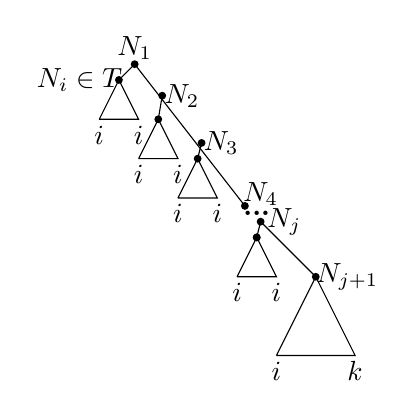
\begin{tikzpicture}
\draw(2.5, 0) -- (3.5,0) -- (3, 1) -- (2.5, 0);
\draw(2, 1) -- (2.5,1) -- (2.25, 1.5) --(2, 1);
\draw(1.25, 2) -- (1.75,2) -- (1.5, 2.5) --(1.25, 2);
\draw(0.75, 2.5) -- (1.25,2.5) -- (1, 3) --(0.75, 2.5);
\draw(0.25, 3) -- (0.75,3) -- (0.5, 3.5) --(0.25, 3);
\draw(3,1) -- (2.3,1.7);
\draw(2.25, 1.5) -- (2.3,1.7);
\draw(2.1, 1.9) -- (0.7, 3.7);

\draw(1.5, 2.5) -- (1.55,2.7);
\draw(1,3) -- (1.05,3.3);
\draw(0.5, 3.5) -- (0.7, 3.7);

\node (start) at (0, 0) {}; 
\node (s) at (2.25 , 1.8) {\textbf{...}}; 
\node (q) at (2.5 , -0.2) {$i$}; 
\node (q2) at (3.5 , -0.2) {$k$}; 
\node (q3) at (2, 0.8) {$i$}; 
\node (q4) at  (2.5,0.8) {$i$}; 
\node (q5) at  (1.25, 1.8) {$i$}; 
\node (q6) at  (1.75,1.8)  {$i$}; 
\node (q7) at  (0.75, 2.3) {$i$}; 
\node (q8) at  (1.25,2.3)  {$i$}; 
\node (q9) at  (0.25, 2.8) {$i$}; 
\node (q10) at  (0.75,2.8)  {$i$}; 

\node (q11) at  (3.4, 1)  {$N_{j+1}$}; 
\node (q11) at  (0.7, 3.9)  {$N_1$}; 
\node (q11) at  (1.3,3.3)  {$N_2$}; 
\node (q11) at  (1.8, 2.7)  {$N_3$}; 
\node (q11) at  (2.6,1.7)  {$N_j$}; 
\node (q11) at  (0, 3.5)  {$N_i \in T$}; 
\node (q11) at  (2.3, 2.05)  {$N_4$}; 


\node [circle, fill=black, inner sep = 1pt, minimum size=0.5pt] at (3, 1) {};
\node [circle, fill=black, inner sep = 1pt, minimum size=0.5pt] at  (2.25, 1.5)  {};
\node [circle, fill=black, inner sep = 1pt, minimum size=0.5pt] at (2.3,1.7) {};
\node [circle, fill=black, inner sep = 1pt, minimum size=0.5pt] at (0.7, 3.7) {};
\node [circle, fill=black, inner sep = 1pt, minimum size=0.5pt] at  (1.55,2.7) {};
\node [circle, fill=black, inner sep = 1pt, minimum size=0.5pt] at  (1.05,3.3) {};
\node [circle, fill=black, inner sep = 1pt, minimum size=0.5pt] at (2.25, 1.5) {};
\node [circle, fill=black, inner sep = 1pt, minimum size=0.5pt] at  (1.5, 2.5) {};
\node [circle, fill=black, inner sep = 1pt, minimum size=0.5pt] at  (1, 3) {};
\node [circle, fill=black, inner sep = 1pt, minimum size=0.5pt] at  (0.5, 3.5) {};
\node [circle, fill=black, inner sep = 1pt, minimum size=0.5pt] at  (2.1, 1.9) {};
\end{tikzpicture}
\\
	\caption{A derivation tree for $l(i \pi k)$, $T \in N$ is the set of terminals.}
\label{partordtree}
\end{figure}


Famous examples of language accepted by partially ordered automata are \textit{piecewise testable languages} \cite*{simon1972hierarchies, masopust2019partially}. A regular language over an alphabet $\Sigma$ is \textit{piecewise testable} if it is a finite Boolean combination of languages of the form $\Sigma^*a_1\Sigma^*a_2\Sigma^* ... \Sigma^*a_k$, where $a_1, a_2, ... , a_k \in \Sigma$, $k \ge 0$. 
\section{Conclusions and open problems}
Metalinear grammars used in DNA computing? --- check it.
For every algebraic number $\alpha$ bigger than 1, a Greibach language whose rational index is in $n^\alpha$ can be found \ref{}. However some context-
free languages with polynomial rational indexes are not Greibach languages \ref{}.
Add to open --- how can we describe all easy CFL? Is it possible?  Seems like not. 
\\Do only stack restictions imply easyness? (bounded stack --- regular languages).
\\Two-counter automaton is powerfull: it can simulate the Turing machine


%\begin{acknowledgements}
%If you'd like to thank anyone, place your comments here
%and remove the percent signs.
%\end{acknowledgements}


% Authors must disclose all relationships or interests that 
% could have direct or potential influence or impart bias on 
% the work: 
%
% \section*{Conflict of interest}
%
% The authors declare that they have no conflict of interest.


% BibTeX users please use one of
%\bibliographystyle{spbasic}      % basic style, author-year citations
%\bibliographystyle{spmpsci}      % mathematics and physical sciences
%\bibliographystyle{spphys}       % APS-like style for physics
%\bibliography{}   % name your BibTeX data base

% Non-BibTeX users please use
%\begin{thebibliography}{}
%
% and use \bibitem to create references. Consult the Instructions
% for authors for reference list style.
%
%\bibitem{RefJ}
% Format for Journal Reference
%Author, Article title, Journal, Volume, page numbers (year)
% Format for books
%\bibitem{RefB}
%Author, Book title, page numbers. Publisher, place (year)
% etc
%\end{thebibliography}
\bibliographystyle{spbasic}      % basic style, author-year citations
\bibliography{paper}   % name your BibTeX data base
\end{document}
% end of file template.tex

